\chapter{Sequential Counters}\label{ch11}
\section{Introduction}

Electronic circuits that require memory devices (like flip-flops or registers) and feedback loops are designed using is called ``Sequential Logic.'' The final output of the circuit is determined by both the inputs and internal circuit feedback loops; and the states of the various logic gates may change rapidly as the output from one stage is fed back to various input points. This makes sequential logic circuits much more dynamic, and complex, than combinational circuits, and their analysis normally requires tools like timing diagrams and state maps. Because sequential circuits are able to latch and hold output states, useful applications like flip-flops, registers, counters, and memory are possible.

%***************************************************************************
% Section: Counters
%***************************************************************************
\section{Counters}
\label{SL:sec:counters}

\subsection{Introduction}
\label{SL:subsec:intro_to_counters}

Counters are a type of sequential circuit designed to count input pulses (normally from a clock) and then activate some output when a specific count is reached. Counters are commonly used as timers; thus, all digital clocks, microwave ovens, and other digital timing displays use some sort of counting circuit. However, counters can be used in many diverse applications. For example, a speed gauge is a counter. By attaching some sort of sensor to a rotating shaft and counting the number of revolutions for $ 60 $ seconds the \gls{rpm} is determined. Counters are also commonly used as frequency dividers. If a high frequency is applied to the input of a counter, but only the ``tens'' count is output, then the input frequency will be divided by ten. As one final example, counters can also be used to control sequential circuits or processes; each count can either activate or deactivate some part of a circuit that controls one of the sequential processes. 

\subsection{Asynchronous Counters}
\label{SL:subsec:asynchronous_counters}

One of the simplest counters possible is an asynchronous two-bit counter. This can be built with a two \emph{JK flip-flops} in sequence, as shown in Figure \ref{fig:09_10}.

\begin{figure}[H]
	\centering
	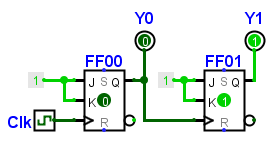
\includegraphics[width=\maxwidth{.95\linewidth}]{gfx/09_10}
	\caption{Asynchronous 2-Bit Counter}
	\label{fig:09_10}
\end{figure}

The J-K inputs on both flip-flops are tied high and the clock is wired into \emph{FF00}. On every positive-going clock pulse the \emph{Q} output for \emph{FF00} toggles and that is wired to the clock input of \emph{FF01}, toggling that output. This type of circuit is frequently called a ``ripple'' counter since the clock pulse must ripple through all of the flip-flops.

In Figure \ref{fig:09_10}, assume both flip-flops start with the output low (or $ 00 $ out). On the first clock pulse, \emph{Q\_FF00} will go high, and that will send a high signal to the clock input of \emph{FF01} which activates \emph{Q\_FF01}. At this point, the \emph{Q} outputs for both flip-flops are high (or $ 11 $ out). On the next clock pulse, \emph{Q\_FF00} will go low, but \emph{Q\_FF01} will not change since it only toggles when the clock goes from low to high. At this point, the output is $ 01 $. On the next clock pulse, \emph{Q\_FF00} will go high and \emph{Q\_FF01} will toggle low: $ 10 $. The next clock pulse toggles \emph{Q\_FF00} to low but \emph{Q\_FF01} does not change: $ 00 $. Then the cycle repeats. This simple circuit counts: $ 00 $, $ 11 $, $ 10 $, $ 01 $. (Note, \emph{Q\_FF00} is the low-order bit.) This counter is counting backwards, but it is a trivial exercise to add the functionality needed to reverse that count.

An asynchronous three-bit counter looks much like the asynchronous two-bit counter, except that a third stage is added.

\begin{figure}[H]
	\centering
	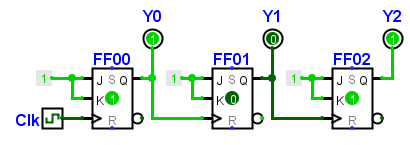
\includegraphics[width=\maxwidth{.95\linewidth}]{gfx/09_11}
	\caption{Asynchronous 3-Bit Counter}
	\label{fig:09_11}
\end{figure}

In Figure \ref{fig:09_11}, the ripple of the clock pulse from one flip-flop to the next is more evident than in the two-bit counter. However, the overall operation of this counter is very similar to the two-bit counter.

More stages can be added so to any desired number of outputs. Asynchronous (or ripple) counters are very easy to build and require very few parts. Unfortunately, they suffer from two rather important flaws:

\begin{itemize}
  \item \textsc{Propagation Delay}. As the clock pulse ripples through the various flip-flops, it is slightly delayed by each due to the simple physical switching of the circuitry within the flip-flop. Propagation delay cannot be prevented and as the number of stages increases the delay becomes more pronounced. At some point, one clock pulse will still be winding its way through all of the flip-flops when the next clock pulse hits the first stage and this makes the counter unstable. 

  \item \textsc{Glitches}. If a three-bit counter is needed, there will be a very brief moment while the clock pulse ripples through the flip-flops that the output will be wrong. For example, the circuit should go from $ 111 $ to $ 000 $, but it will actually go from $ 111 $ to $ 110 $ then $ 100 $ then $ 000 $ as the ``low'' ripples through the flip-flops. These glitches are very short, but they may be enough to introduce errors into a circuit.
\end{itemize}

Figure \ref{fig:09_12} is a four-bit asynchronous counter.

\begin{figure}[H]
	\centering
	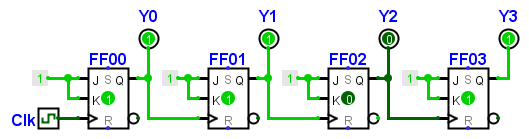
\includegraphics[width=\maxwidth{.95\linewidth}]{gfx/09_12}
	\caption{Asynchronous 4-Bit Counter}
	\label{fig:09_12}
\end{figure}

Figure \ref{tmg:09_07} is the timing diagram obtained when the counter in Figure \ref{fig:09_12} is executing.

\begin{figure}[H]
  \centering
  \begin{tikztimingtable}[
    timing/slope=0,         % no slope
    timing/coldist=2pt,     % column distance
    xscale=1.0,yscale=1.0,  % scale diagrams
    semithick,               % set line width
    ]
    \footnotesize \# & U     R 18{2Q} 2U     \\
    \footnotesize Clk & 36{C} \\
    %                      P 01 02 03 04 05 06 07 08 09 10 11 12 13 14 15 16 17 18
    \footnotesize Y0 & [] {L HH LL HH LL HH LL HH LL HH LL HH LL HH LL HH LL HH LL} \\
    \footnotesize Y1 & [] {L HH HH LL LL HH HH LL LL HH HH LL LL HH HH LL LL HH HH} \\
    \footnotesize Y2 & [] {L HH HH HH HH LL LL LL LL HH HH HH HH LL LL LL LL HH HH} \\
    \footnotesize Y3 & [] {L HH HH HH HH HH HH HH HH LL LL LL LL LL LL LL LL HH HH} \\
    \extracode % Optional
    % \fulltablegrid[]
    % \vertlines[]{}
    \tablerules[]
  \end{tikztimingtable}
  \caption{4-Bit Asynchronous Counter Timing Diagram} 
  \label{tmg:09_07}
\end{figure}

Notice that \emph{Y0} counts at half the frequency of the clock and then \emph{Y1} counts at half that frequency and so forth. Each stage that is added will count at half the frequency of the previous stage.

\subsection{Synchronous Counters}
\label{SL:subsec:synchronous_counters}

Both problems with ripple counters can be corrected with a synchronous counter, where the same clock pulse is applied to every flip-flop at one time. Here is the logic diagram for a synchronous two-bit counter: 

\begin{figure}[H]
	\centering
	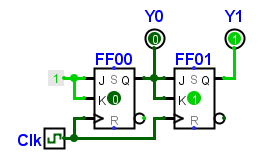
\includegraphics[width=\maxwidth{.95\linewidth}]{gfx/09_13}
	\caption{Synchronous 2-Bit Counter}
	\label{fig:09_13}
\end{figure}

Notice in this circuit, the clock is applied to both flip-flops and control is exercised by applying the output of one stage to both $ J $ and $ K $ inputs of the next stage, which effectively enables/disables that stage. When Q\_FF00 is high, for example, then the next clock pulse will make FF01 change states. 

\begin{figure}[H]
	\centering
	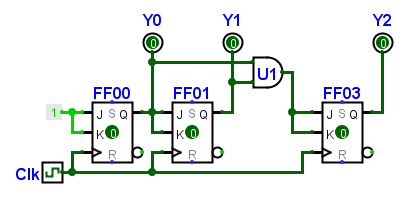
\includegraphics[width=\maxwidth{.95\linewidth}]{gfx/09_14}
	\caption{Synchronous 3-Bit Counter}
	\label{fig:09_14}
\end{figure}

A three-bit synchronous counter applies the clock pulse to each flip-flop. Notice, though, that the output from the first two stages must routed through an \textsf{AND} gate so \emph{FF03} will only change when \emph{Q\_FF00} and \emph{Q\_FF01} are high. This circuit would then count properly from $ 000 $ to $ 111 $. 

In general, synchronous counters become more complex as the number of stages increases since it must include logic for every stage to determine when that stage should activate. This complexity results in greater power usage (every additional gate requires power) and heat generation; however, synchronous counters do not have the propagation delay problems found in asynchronous counters. 

\begin{figure}[H]
	\centering
	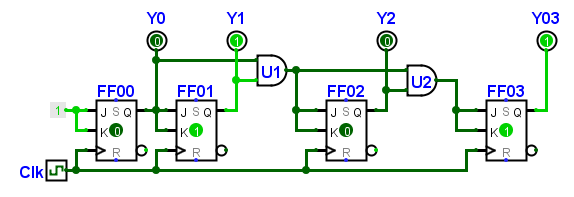
\includegraphics[width=\maxwidth{.95\linewidth}]{gfx/09_15}
	\caption{Synchronous 4-Bit Up Counter}
	\label{fig:09_15}
\end{figure}

Figure \ref{tmg:09_08} is the timing diagram for the circuit illustrated in Figure \ref{fig:09_15}.

\begin{figure}[H]
  \centering
  \begin{tikztimingtable}[
    timing/slope=0,         % no slope
    timing/coldist=2pt,     % column distance
    xscale=1.0,yscale=1.0,  % scale diagrams
    semithick,               % set line width
    ]
    \footnotesize \# & U     R 18{2Q} 2U     \\
    \footnotesize Clk & 36{C} \\
    %                      P 01 02 03 04 05 06 07 08 09 10 11 12 13 14 15 16
   %17 18
    \footnotesize Y0 & [] {L HH LL HH LL HH LL HH LL HH LL HH LL HH LL HH LL HH LL} \\
    \footnotesize Y1 & [] {L LL HH HH LL LL HH HH LL LL HH HH LL LL HH HH LL LL HH} \\
    \footnotesize Y2 & [] {L LL LL LL HH HH HH HH LL LL LL LL HH HH HH HH LL LL LL.} \\
    \footnotesize Y3 & [] {L LL LL LL LL LL LL LL HH HH HH HH HH HH HH HH LL LL LL} \\
    \extracode % Optional
    % \fulltablegrid[]
    % \vertlines[]{}
    \tablerules[]
  \end{tikztimingtable}
  \caption{4-Bit Synchronous Counter Timing Diagram} 
  \label{tmg:09_08}
\end{figure}

The timing diagram for the asynchronous counter in Figure \ref{tmg:09_07} is the same as that for an synchronous counter in Figure \ref{tmg:09_08} since the output of the two counters are identical. The only difference in the counters is in how the count is obtained, and designers would normally opt for a synchronous \gls{ic} since that is a more efficient circuit.

\subsubsection{Synchronous Down Counters}
\label{SL:subsubsec:synchronous_down_counters}

It is possible to create a counter that counts down rather than up by using the \emph{Q'} outputs of the flip-flops to trigger the next stage. Figure \ref{fig:09_16} illustrates a four-bit down counter.

\begin{figure}[H]
	\centering
	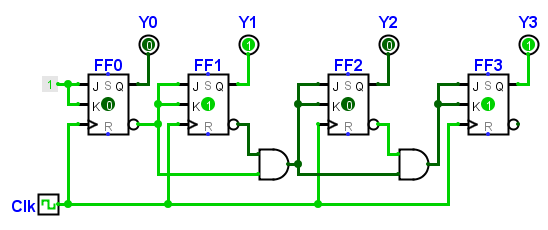
\includegraphics[width=\maxwidth{.95\linewidth}]{gfx/09_16}
	\caption{Synchronous 4-Bit Down Counter}
	\label{fig:09_16}
\end{figure}

Figure \ref{tmg:09_09} is the timing diagram for the circuit illustrated in Figure \ref{fig:09_16}.

\begin{figure}[H]
	\centering
	\begin{tikztimingtable}[
		timing/slope=0,         % no slope
		timing/coldist=2pt,     % column distance
		xscale=1.0,yscale=1.0,  % scale diagrams
		semithick,               % set line width
		]
		\footnotesize \# & U     R 18{2Q} 2U     \\
		\footnotesize Clk & 36{C} \\
		%                      P 01 02 03 04 05 06 07 08 09 10 11 12 13 14 15 16
	 %17 18
		\footnotesize Y0 & [] {L HH LL HH LL HH LL HH LL HH LL HH LL HH LL HH LL HH LL} \\
		\footnotesize Y1 & [] {L HH HH LL LL HH HH LL LL HH HH LL LL HH HH LL LL HH HH} \\
		\footnotesize Y2 & [] {L HH HH HH HH LL LL LL LL HH HH HH HH LL LL LL LL HH HH} \\
		\footnotesize Y3 & [] {L HH HH HH HH HH HH HH HH LL LL LL LL LL LL LL LL HH HH} \\
		\extracode % Optional
		% \fulltablegrid[]
		% \vertlines[]{}
		\tablerules[]
	\end{tikztimingtable}
	\caption{4-Bit Synchronous Down Counter Timing Diagram} 
	\label{tmg:09_09}
\end{figure}


\subsection{Ring Counters}
\label{SL:subsec:ring_counters}

A ring counter is a special kind of counter where only one output is active at a time. As an example, a four-bit ring counter may output this type of pattern:

\medskip
\texttt{ $ 1000 - 0100 - 0010 - 0001 $ }
\medskip

Notice the high output cycles through each of the bit positions and then recycles. Ring counters are useful as controllers for processes where one process must follow another in a sequential manner. Each of the bits from the ring counter can be used to activate a different part of the overall process; thus ensuring the process runs in proper sequence. The circuit illustrated in Figure \ref{fig:09_17} is a 4-bit ring counter.

\begin{figure}[H]
	\centering
	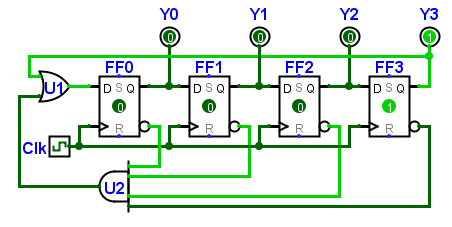
\includegraphics[width=\maxwidth{.95\linewidth}]{gfx/09_17}
	\caption{4-Bit Ring Counter}
	\label{fig:09_17}
\end{figure}

When the circuit is initialized none of the flip-flops are active. Because \emph{Q'} is high for all flip-flops, \textsf{AND} gate \emph{U2} is active and that sends a high through \emph{U1} and into the data port of \emph{FF0}. The purpose of \emph{U2} is to initialize \emph{FF0} for the first count and then \emph{U2} is never activated again. On each clock pulse the next flip-flop in sequence is activated. When \emph{FF3} is active that output is fed back through \emph{U1} to \emph{FF0}, completing the ring and re-starting the process.

Figure \ref{tmg:09_10} is the timing diagram for the ring counter illustrated in Figure \ref{fig:09_17}.

\begin{figure}[H]
  \centering
  \begin{tikztimingtable}[
    timing/slope=0,         % no slope
    timing/coldist=2pt,     % column distance
    xscale=2.0,yscale=1.0,  % scale diagrams
    semithick,               % set line width
    ]
    \footnotesize \# & U     R 8{2Q} 2U     \\
    \footnotesize Clk & 17{C} \\
    %                        P 01 02 03 04 05 06 07 08
    \footnotesize Y0 & [] {L HH LL LL LL HH LL LL LL} \\
    \footnotesize Y1 & [] {L LL HH LL LL LL HH LL LL} \\
    \footnotesize Y2 & [] {L LL LL HH LL LL LL HH LL} \\
    \footnotesize Y3 & [] {L LL LL LL HH LL LL LL HH} \\
    \extracode % Optional
    % \fulltablegrid[]
    % \vertlines[]{}
    \tablerules[]
  \end{tikztimingtable}
  \caption{4-Bit Ring Counter Timing Diagram} 
  \label{tmg:09_10}
\end{figure}

On each clock pulse a different bit is toggled high, proceeding around the four-bit nibble in a ring pattern.

\subsubsection{Johnson Counters}
\label{SL:subsubsec:johnson_counters}

One common modification of a ring counter is called a Johnson, or ``Twisted Tail,'' ring counter. In this case, the counter outputs this type of pattern.

\medskip
\texttt{ $ 1000 - 1100 - 1110 - 1111 - 0111 - 0011 - 0001 - 0000 $ }
\medskip

The circuit illustrated in Figure \ref{fig:09_18} is a 4-bit Johnson counter.

\begin{figure}[H]
	\centering
	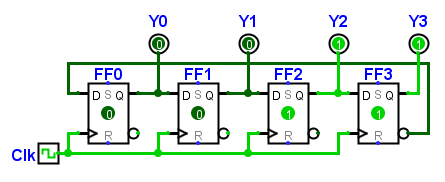
\includegraphics[width=\maxwidth{.95\linewidth}]{gfx/09_18}
	\caption{4-Bit Johnson Counter}
	\label{fig:09_18}
\end{figure}

This is very similar to the ring counter except the feedback loop is from \emph{Q'} rather than \emph{Q} of \emph{FF3} and because of that, the \textsf{AND} gate initialization is no longer needed. 

Figure \ref{tmg:09_11} is the timing diagram for the Johnson counter illustrated in Figure \ref{fig:09_18}.

\begin{figure}[H]
	\centering
	\begin{tikztimingtable}[
		timing/slope=0,         % no slope
		timing/coldist=2pt,     % column distance
		xscale=1.0,yscale=1.0,  % scale diagrams
		semithick,               % set line width
		]
		
    \footnotesize \# & U     R 18{2Q} 2U     \\
\footnotesize Clk & 36{C} \\
%                          P 01 02 03 04 05 06 07 08 09 10 11 12 13 14 15 16
%   17 18		
		\footnotesize Y0 & [] {L HH HH HH HH LL LL LL LL HH HH HH HH LL LL LL LL  HH H} \\
		\footnotesize Y1 & [] {L LL HH HH HH HH LL LL LL LL HH HH HH HH LL LL LL LL H} \\
		\footnotesize Y2 & [] {L LL LL HH HH HH HH LL LL LL LL HH HH HH HH LL LL LL L} \\
		\footnotesize Y3 & [] {L LL LL LL HH HH HH HH LL LL LL LL HH HH HH HH LL LL L} \\
		\extracode % Optional
		% \fulltablegrid[]
		% \vertlines[]{}
		\tablerules[]
	\end{tikztimingtable}
	\caption{4-Bit Johnson Counter Timing Diagram} 
	\label{tmg:09_11}
\end{figure}

\subsection{Modulus Counters}
\label{SL:subsec:modulus_counters}

Each of the counters created so far have had one significant flaw, they only count up to a number that is a power of two. A two-bit counter counts from zero to three, a three-bit counter counts from zero to seven, a four-bit counter counts from zero to $ 15 $, and so forth. With a bit more work a counter can be created that stops at some other number. These types of counters are called ``modulus counters'' and an example of one of the most common modulus counters is a decade counter that counts from zero to nine. The circuit illusted in Figure \ref{fig:09_19} is a decade counter.

\begin{figure}[H]
	\centering
	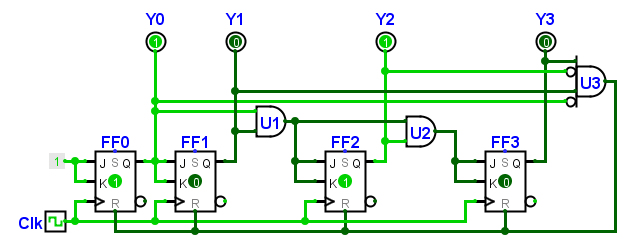
\includegraphics[width=\maxwidth{.95\linewidth}]{gfx/09_19}
	\caption{Decade Counter}
	\label{fig:09_19}
\end{figure}

This is only a four-bit counter (found in Figure \ref{fig:09_15}) but with an additional \textsf{AND} gate (\emph{U3}). The inputs for that \textsf{AND} gate are set such that when \emph{Y0}-\emph{Y3} are $ 1010 $ then the gate will activate and reset all four flip-flops.

Figure \ref{tmg:09_12} is the timing diagram obtained from the decade counter illustrated in Figure \ref{fig:09_19}.

\begin{figure}[H]
	\centering
	\begin{tikztimingtable}[
		timing/slope=0,         % no slope
		timing/coldist=2pt,     % column distance
		xscale=1.0,yscale=1.0,  % scale diagrams
		semithick,               % set line width
		]
		\footnotesize \# & U     R 18{2Q} 2U     \\
		\footnotesize Clk & 36{C} \\
		%                      P 01 02 03 04 05 06 07 08 09 10 11 12 13 14 15 16
	 %17 18
		\footnotesize Y0 & [] {L HH LL HH LL HH LL HH LL HH LL HH LL HH LL HH LL HH LL} \\
		\footnotesize Y1 & [] {L LL HH HH LL LL HH HH LL LL LL HH HH LL LL HH HH LL LL} \\
		\footnotesize Y2 & [] {L LL LL LL HH HH HH HH LL LL LL LL LL HH HH HH HH LL LL} \\
		\footnotesize Y3 & [] {L LL LL LL LL LL LL LL HH HH LL LL LL LL LL LL LL HH HH} \\
		\extracode % Optional
		% \fulltablegrid[]
		\vertlines[]{19}
		\tablerules[]
	\end{tikztimingtable}
	\caption{4-Bit Decade Counter Timing Diagram} 
	\label{tmg:09_12}
\end{figure}

The timing diagram shows the count increasing with each clock pulse (for example, at $ 8 $ the outputs are $ 1000 $) until pulse number ten, when the bits reset to $ 0000 $ and the count starts over. A vertical line was added at count ten for reference.

\subsection{Up-Down Counters}
\label{SL:subsec:up_down_counters}

In this chapter both up and down counters have been considered; however counters can also be designed to count both up and down. These counters are, of course, more complex than the simple counters encountered so far and Figure \ref{fig:09_20} illustrates an up-down counter circuit.

\begin{figure}[H]
	\centering
	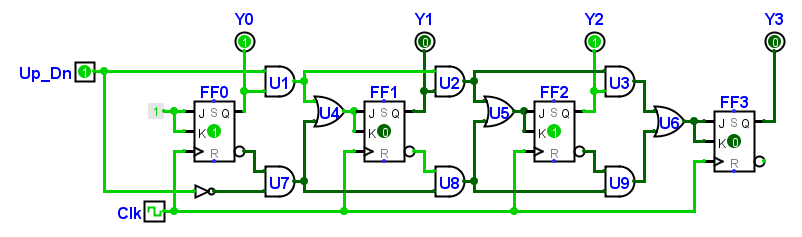
\includegraphics[width=\maxwidth{.95\linewidth}]{gfx/09_20}
	\caption{Up-Down Counter}
	\label{fig:09_20}
\end{figure}

When the \emph{Up\_Dn} bit is high the counter counts up but when that bit is low then the counter counts down. This counter is little more than a merging of the up counter in Figure \ref{fig:09_15} and the down counter in Figure \ref{fig:09_16}. \emph{U1}-\emph{U3} transmit the \emph{Q} outputs from each flip-flop to the next stage while \emph{U7}-\emph{U9} transmit the \emph{Q'} outputs from each flip-flop to the next stage. The E bit activates one of those two banks of \textsf{AND} gates.

No timing diagram is provided for this circuit since that diagram would be the same as for the up counter (Figure \ref{tmg:09_08} or the down counter (Figure \ref{tmg:09_09}), depending on the setting of the \emph{Up\_Dn} bit.

\subsection{Frequency Divider}
\label{SL:subsec:frequency_divider}

Often, a designer creates a system that may need various clock frequencies throughout its subsystems. In this case, it is desirable to have only one main pulse generator, but divide the frequency from that generator so other frequencies are available where they are needed. Also, by using a common clock source all of the frequencies are easier to synchronize when needed.

The circuit illustrated in Figure \ref{fig:09_21} is the same synchronous two-bit counter first considered in Figure \ref{fig:09_13}.

\begin{figure}[H]
	\centering
	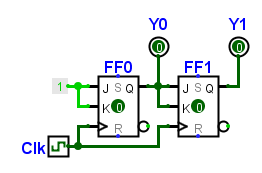
\includegraphics[width=\maxwidth{.95\linewidth}]{gfx/09_21}
	\caption{Synchronous 2-Bit Counter}
	\label{fig:09_21}
\end{figure}

The circuit in Figure \ref{fig:09_21} produces the timing diagram seen in Figure \ref{tmg:09_13}
 
\begin{figure}[H]
  \centering
  \begin{tikztimingtable}[
    timing/slope=0,         % no slope
    timing/coldist=2pt,     % column distance
    xscale=2.0,yscale=1.0,  % scale diagrams
    semithick,               % set line width
    ]
    \footnotesize \# & U     R 8{2Q} 2U     \\
    \footnotesize Clk & 17{C} \\
    %                 P 01 02 03 04 05 06 07 08
    \footnotesize Y0 & [] {L HH LL HH LL HH LL HH LL} \\
    \footnotesize Y1 & [] {L HH HH LL LL HH HH LL LL} \\
    \extracode % Optional
    % \fulltablegrid[]
    % \vertlines[]{}
    \tablerules[]
  \end{tikztimingtable}
  \caption{Frequency Divider} 
  \label{tmg:09_13}
\end{figure}

Notice that \emph{Y0} is half of the clock's frequency and \emph{Y1} is one-quarter of the clock's frequency. If the circuit designer used Y1 as a timer for some subcircuit then that circuit would operate at one-quarter of the main clock frequency. It is possible to use only one output port from a modulus counter, like the decade counter found in Figure \ref{fig:09_19}, and get any sort of division of the main clock desired.

\subsection{Counter Integrated Circuits (IC)}
\label{SL:subsec:counter_integrated_circuits}

In practice, most designers do not build counter circuits since there are so many types already commercially available. When a counter is needed, a designer can select an appropriate counter from those available on the market. Here are just a few as examples of what is available: 

\begin{table}[H]
  \sffamily
  \newcommand{\head}[1]{\textcolor{white}{\textbf{#1}}}    
  \begin{center}
    \rowcolors{2}{gray!10}{white} % Color every other line a light gray
    \begin{tabular}{ll} 
      \rowcolor{black!75}
      \head{IC} & \head{Function} \\
      74x68 & dual four-bit decade counter \\
      74x69 & dual four-bit binary counter \\
      74x90 & decade counter (divide by $ 2 $ and divide by $ 5 $ sections) \\
      74x143 & decade counter/latch/decoder/seven-segment driver \\
      74x163 & synchronous four-bit binary counter \\
      74x168 & synchronous four-bit up/down decade counter \\
      74x177 & presettable binary counter/latch \\
      74x291 & four-bit universal shift register and up/down counter
    \end{tabular}
  \end{center}
  \caption{Counter IC's}
  \label{sl:tab:counter_ics}
\end{table}

\section{Memory}
\label{SL:sec:memory}

\subsection{Read-Only Memory}
\label{SL:subsec:read-only_memory}

\gls{rom} is an \gls{ic} that contains tens-of-millions of registers (memory locations) to store information. Typically, \gls{rom} stores microcode (like bootup routines) and computer settings that do not change. There are several types of \gls{rom}: mask, programmable, and erasable. 

\begin{itemize}
  \item \textsc{Mask} \glspl{rom} are manufactured such that memory locations already filled with data and that cannot be altered by the end user. They are called ``mask'' \glspl{rom} since the manufacturing process includes applying a mask to the circuit as it is being created. 
  \item \textsc{\glspl{prom}} are a type of \gls{rom} that can be programmed by the end user, but it cannot be altered after that initial programming. This permits a designer to distribute some sort of program on a chip that is designed to be installed in some device and then never changed.
  \item \textsc{Erasable \glspl{prom}} can be programmed by the end user and then be later altered. An example of where an erasable \gls{prom} would be used is in a computer's \gls{bios} (the operating system that boots up a computer), where the user can alter certain ``persistent'' computer specifications, like the device boot order. 
\end{itemize}

Two major differences between \gls{rom} and \gls{ram} are 1) \gls{rom}'s ability to hold data when the computer is powered off and 2) altering the data in \gls{ram} is much faster than in an erasable \gls{prom}.

\subsection{Random Access Memory}
\label{SL:subsec:random_access_memory}

\gls{ram} is an integrated circuit that contains tens-of-millions of registers (memory locations) to store information. The \gls{ram} \gls{ic} is designed to quickly store data found at its input port and then look-up and return stored data requested by the circuit. In a computer operation, \gls{ram} contains both program code and user input (for example, the \emph{LibreOffice Writer} program along with whatever document the user is working on). There are two types of \gls{ram}: dynamic and static. \gls{dram} stores bits in such a way that it must be ``refreshed'' (or ``strobed'') every few milliseconds. \gls{sram} uses flip-flops to store data so it does not need to be refreshed. One enhancement to \glspl{dram} was to package several in a single \gls{ic} and then synchronize them so they act like a single larger memory; these are called \glspl{sdram} and they are very popular for camera and cell phone memory.

Both \gls{rom} and \gls{ram} circuits use registers, flip-flops, and other components already considered in this chapter, but by the millions rather than just four or so at a time. There are no example circuits or timing diagrams for these devices in this book; however, the lab manual that accompanies this book includes activities for both \gls{rom} and \gls{ram} devices.

















